\documentclass{beamer}
\title{Extending Zero Trust architecture to Kubernetes sidecars}
\author{Aarni Halinen}
\institute{
  Department of Computer Science\\
  Aalto University
}
\date{\today}

\begin{document}

\frame{
  \titlepage

  Supervisor: Prof.\ Mario Di Francesco
  \\
  Advisor: M.Sc.\ (Tech.)\ José\ Luis\ Martin\ Navarro
  \\
  Advisor: M.Sc.\ (Tech.)\ Jacopo\ Bufalino
}

\frame{
  \frametitle{Contents}

  \begin{enumerate}
    \item Zero Trust Architecture
    \item Kubernetes: sidecars and networking model
    \item Research: threat modelling and mitigation
    \item Future considerations
  \end{enumerate}
}

\frame{
  \frametitle[ZTA]{Zero Trust Architecture}

  \emph{A security paradigm that focuses on the premise that trust must always be explicitly granted}

  \begin{itemize}
    \item Move security boundaries to the most granular level and use fine-grained access rules
    \item A multi-layer, defense-in-depth approach
    \item Network communication, even if internal and behind a firewall, should not be trusted
    \item Services communicate securely (Mutual authentication, with mTLS), rely on more robust identifiers than IP addresses, and restrict traffic on L5-L7
    \item Modern service meshes help implementing the architecture in Kubernetes clusters, often using sidecars (like Envoy proxy)
  \end{itemize}
}

\frame{
  \frametitle{Kubernetes sidecars}

  \begin{itemize}
    \item Sidecar pattern allows isolating of peripheral tasks (logging, observability, Envoy proxies) from application to own helper containers called sidecars
    \item Pods consist of one or more tightly-coupled containers, sidecars are not technically distinguishable from application container
    \item Containers in Pod share Linux network namespace with each other
  \end{itemize}
}

\frame{
  \frametitle{K8s networking model}

  \begin{itemize}
    \item Addresses 4 different types of networking communication
    \begin{itemize}
      \item Inside Pod's network namespace (localhost)
      \item Pod-to-Pod, even accross different Nodes
      \item Service-to-Pod
      \item Cluster external sources to Services
    \end{itemize}
    \item Pod-to-Pod connection is implemented by a CNI plugin that creates NIC and assigns IP addresses (IPAM)
    \item CNI plugins with operator daemons can also implement network rules (Network Policy resource)
    \item Calico, Cilium
    \item Meta-plugins such as Multus implement other features as part of the CNI chain
  \end{itemize}
}

\frame{
  \frametitle{Sidecar threat modelling}

  \begin{figure}[h!]
    \centering
    \includegraphics[width=\linewidth]{../thesis/files/Matrix copy.png}
    \caption{Kubernetes threat matrix (MITRE ATT\&CK) [2]}
  \end{figure}

  \begin{itemize}
    \item Initial access is already assumed
    \item Attacks are also experimented with custom container in a Minikube cluster
  \end{itemize}
}

\frame{
  \frametitle{Permission related threats}

  \begin{itemize}
    \item Most of the threats found are easily mitigated with Pod Security Admission Controller
    \item Other threats can be mitigated with custom admission controllers
    \begin{itemize}
      \item Containers in a Pod share and automatically mount Service Accounts $\Rightarrow$ do not allow automatic SA mounting, manually mount to containers when needed
      \item Resource limits are not enforced (denial of service) $\Rightarrow$ enforce with admission webhooks
    \end{itemize}
  \end{itemize}
}

\frame{
  \frametitle{Networking threats}

  \begin{itemize}
    \item The common network namespace in Pod's allows unlimited access to other containers
    \item Network policies apply to all containers in a Pod
    \item No built-in options for fine-grained network access within the network namespace
    \item Two different approaches invistigated
    \item Both approaches should not interfere with permission related mitigations
  \end{itemize}
}

\frame{
  \frametitle{Approach 1: Injecting networking rules to Pod}

  \begin{figure}[h!]
    \centering
    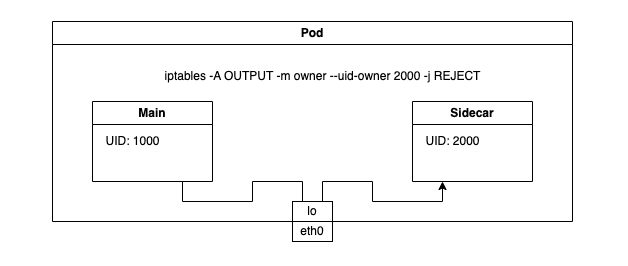
\includegraphics[width=\linewidth]{../thesis/files/iptables.png}
  \end{figure}

  \begin{itemize}
    \item Inject IPTables rules to Pod net namespace after deployment
    \item Containers are distinguished from one another by using unique user IDs and IPTables owner-module
  \end{itemize}
}

\frame{
  \frametitle{Approach 2: Split the Pod and rebuild sidecar-like connectivity}

  \begin{figure}[h!]
    \centering
    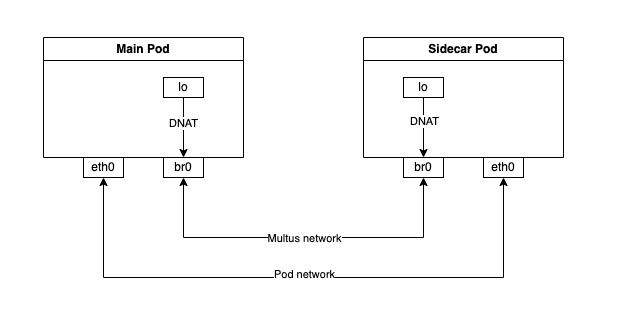
\includegraphics[width=\linewidth]{../thesis/files/multus.png}
  \end{figure}

  \begin{itemize}
    \item All containers are inherently in own net NS
    \item Multus used for static IPs, NPs and isolation from Pod network
    \item Loopback connectivity with \texttt{net.ipv4.conf.all.route\_localnet=1}
  \end{itemize}
}

\frame{
  \frametitle{Findings}

  \begin{itemize}
    \item Moving security boundaries to container-level is possible, but laborous to implement
    \begin{itemize}
      \item Keeping access rules up-to-date requires a custom K8s operator
      \item Multus is not yet a mature project
      \item Multus approach breaks co-scheduling
      \item mTLS between containers is not solved
    \end{itemize}
    \item \emph{Avoiding sidecars is the best mitigation}
    \item $\Rightarrow$ Use DaemonSets to run sidecars per-Node
  \end{itemize}
}

\frame{
  \frametitle{Future development}

  \begin{itemize}
    \item K8s v1.28 introduces SidecarContainers
    \begin{itemize}
      \item Introduced for fixing existing lifecycle issues of initContainers
      \item Proposal explicitly states a non-goal of enforcing different security regulations for sidecars
    \end{itemize}
    \item Service meshes have introduced sidecarless architectures
    \item Cilium service mesh (eBPF) and Istio ambient mesh
  \end{itemize}
}

\frame{
\frametitle{Re-cap}

\begin{figure}[h!]
  \centering
  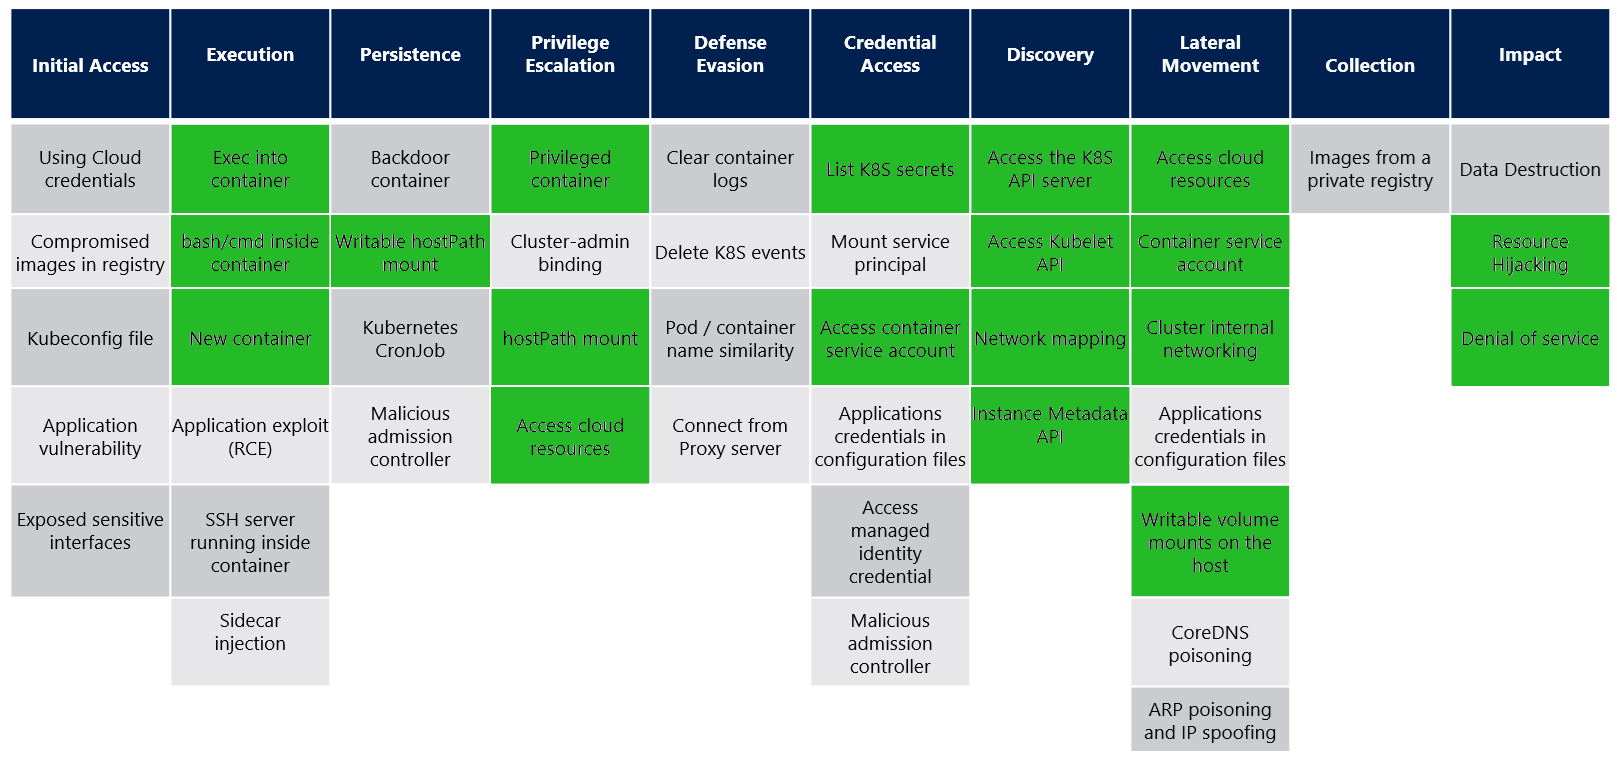
\includegraphics[width=\linewidth]{../thesis/files/Matrix.png}
  \caption{Threat matrix. Attack techniques addressed are highlighted in green.}
\end{figure}
}

\frame{
  \frametitle{Re-cap}

  \begin{itemize}
    \item The thesis investigated and found ways to mitigate sidecar related threats in K8s
    \item Most vulnerable configuration can be prevented with PSA
    \item Admission controller allows extending protections even further
    \item No existing way to implement ZTA in sidecar networking, but it is possible
    \item Implementing the network solutions are cumbersome and require extensive work
    \item Avoiding sidecars altogether is the easiest mitigation
  \end{itemize}
}

\frame{
  \frametitle{References}

  \begin{itemize}
    \item [1] Kubernetes components, Kubernetes documentation.
    [https://kubernetes.io/docs/concepts/overview/components/]
    \item [2] Secure containerized environments with updated threat matrix for Kubernetes, By Yossi Weizman, Senior Security Researcher, Microsoft Defender for Cloud.
    [https://www.microsoft.com/en-us/security/blog/2021/03/23/secure-containerized-environments-with-updated-threat-matrix-for-kubernetes/]
  \end{itemize}
}

\end{document}
